\documentclass[../Text/00main.tex]{subfiles}
\graphicspath{{../}}

\begin{document}

% meer over sorensen
%!!! dat 1D model even vinden!!

\section{Simulation setup}




\subsection{Software \& Hardware}

The software used for the earthquake simulations in this research is Salvus, a high-performance sorftware suite developed by Mondaic \cite{afanasiev_modular_2019}. This spectral-element wavefield solver has an extensive set of features and a wide range of applications, from small-scale medical imaging applications to large-scale global wavefield simulations. Processing of the simulated wavefields was mainly done using Obspy. Appendix \ref{app:software} gives an overview of the used packages for this research. 

Simulations up to a period of $T = 4 s$ could be run on a local machine for the regional simulations run in this study. However, for the simulations of $T < 4 s s$ use was made of the CSCS Piz Daint HPC. The main specifications for this machine can be found in Appendix Table \ref{app:pizdaint}. 


\subsection{Databases}

% iets over mb, ml etc??

In order to assess the performance of the model with respect to reality, simulations could be compared to real data. Event data in this report comes from the IRIS catalogue (FSDN). Information about the focal mechanisms of these events was taken from the GCMT catalogue (\cite{dziewonski_determination_1981}, \cite{ekstromdziewo}). For two small events, the GFZ World Stress Map 2016 (wsm2016, \cite{heidbach2016world}) was consulted.

\subsection{Models}

\subsubsection{Model of Turkey}

The main reference model in this study, is the three-dimensional \textit{csem\_eastmed} model which is described in \cite{cubuk-sabuncu_3-d_2017}. This model was constructed using full-waveform inversion of 62 regional events, and is accurate up to a period of $T = 8 s$. It is used as the volume model for the mantle in the simulations, and dictates the VHS and VPH velocities. An additional 1D model is also considered in this study, to see whether usage of a complex 3D volume model is significantly improving the results. The 1D model is adapted from the 1D model used in \cite{pulido_sensitivity_2007} and the anisotropic PREM model. 

\hl{To do: insert small graph of 1D model with depth}

% find model

\subsubsection{Source time function}

\begin{figure}[h!]
    \centering
    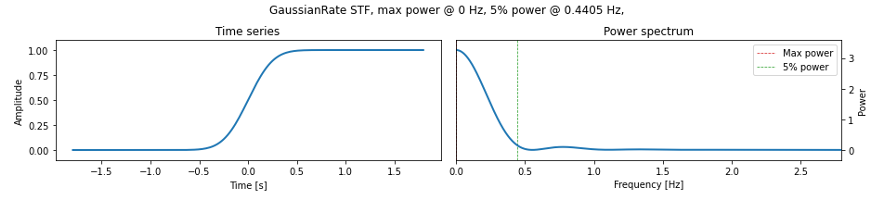
\includegraphics{images_methods/GR_stf_image.png}
    \caption{Time series (left) and power spectrum (right) of a Gaussian rate source-time function at a minimum period of $ T=1 s$.}
    \label{fig:Gaussian_rate_stf}
\end{figure}

The rupture of the source is modelled as a source-time function $s(t)$. The source-time function in this study is a\textit{ Gaussian rate}, which models for the first time derivative of a Gaussian: 

\begin{equation}
s(t)=\frac{1}{2}+\frac{1}{\sqrt{\pi}} \int_{t_{0}}^{t} \exp \left(-\frac{\alpha\left(t-t_{0}\right)}{\tau}\right)^{2} dt , 
\label{eq:Gaussianrate}
\end{equation}

with period $\tau$, time $t$ and time shift $t_0$, and $\alpha$ as the decay rate.  

The Gaussian rate represents the physical slip rate or moment rate, and is one of the built-in source-time functions in Salvus. It is often used in rupture simulation because of the intuitive connection between moment rate and a physical rupture. 

Another option is directly using a Ricker wavelet as source-time function:

\begin{figure}[h!]
    \centering
    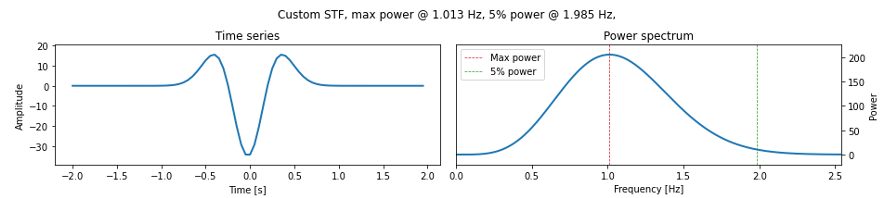
\includegraphics{images_methods/custom_stf.png}
    \caption{Time series (left) and power spectrum (right) of a custom Ricker wavelet source-time function at a minimum period of $ T=1 s$.}
    \label{fig:Custom_stf}
    \label{eq:custom}
\end{figure}



\begin{equation}
s(t)=\left(1-2\left(t-t_{0}\right)^{2} \pi^{2} \omega^{2}\right) \exp \left(-\left(t-t_{0}\right)^{2} \pi^{2} \omega^{2}\right),
\end{equation}

with $\omega$ the centre frequency of the wavelet.

%reference

Using the Ricker wavelet as source time function comes with the advantage that the time-stepping scheme allows for a slightly higher accuracy. Because the output traces of simulations using the Ricker wavelet are the second derivative of the Gaussian, the result has to be integrated with respect to time three times to model displacement, twice to model velocity and once for acceleration. One run is done to test whether using this function and thus allowing for slightly higher precision, affects the distribution of ground motion proxies. 

\subsubsection{Topography and bathymetry model}


% Topography from ...

The topography model in this study is an absolute surface model constructed by combination of the geoid by \cite{pavlis2012development} and bedrock topography, bathymetry and ice by \cite{hirt2015earth2014}. For the bathymetry in our model, the difference between the bedrock topography, bathymetry and ice model (referred to as Earth2014\_TBI by Mondaic), and the surface Earth2014\_SUR model. Resolution of these models is given in angular order. We use the highest angular order models, with an order of 10800, corresponding to a spatial resolution of 1.8 km. 

[image of domain with topography]

\subsubsection{Ocean model}

Salvus offers the possibility of implementing two types of ocean effects in the domain. Either an oceanic load, or an accoustic ocean with coupling between the solid surface and fluid can be implemented. The latter only differs significantly from the ocean loading if the ocean depth is at least 10\% of the minimum wavelength, and it is advised to model the ocean up to 1/4th of the minimum wavelength in the domain. In this case, the minimum velocity in the domain is in the ocean, at $v_{min} = 1450 m/s$. In shallower regions than this criterium, an ocean load is applied. The simulations including ocean coupling are modeled at a frequency of $1 Hz$, and so this cut-off  depth was set at 300 m. Because of the steep bathymetry just offshore of Istanbul, this cutoff coincides here with the steep underwater cliffs. 


[image of domain with ocean]


\subsubsection{Domain}

Two regions of the model are explored. For the validation phase a large (300 x 200 km) domain is considered for lower-frequency tests, and a sub-domain of this region (100 x 80 km) is considered for testing the model up to a frequency of 1 Hz. The model domain for the main simulations in this research is situated near Istanbul. Properties are listed in Table \ref{tab:Domainsizes} and visualisations in \hl{To do: add paraview images of domain}. 

% Please add the following required packages to your document preamble:
% \usepackage{booktabs}
% \usepackage[normalem]{ulem}
% \useunder{\uline}{\ul}{}
\begin{table}[]
\caption{Domain information. Number of points and elements vary per frequency for the Çubuk domain. }
\begin{tabular}{@{}lcclllll@{}}
\toprule
 &
  \multicolumn{4}{c}{\textbf{Istanbul simulation}} &
  \multicolumn{3}{c}{\textbf{Çubuk validations}} \\ \midrule
\multicolumn{1}{l|}{} &
  \multicolumn{1}{l|}{3D} &
  \multicolumn{1}{c|}{1D} &
  \multicolumn{1}{l|}{3D + topo} &
  \multicolumn{1}{l|}{3D + topo + ocean} &
  \multicolumn{1}{l|}{3D large} &
  \multicolumn{1}{l|}{1D large} &
  3D small \\ \midrule
\multicolumn{1}{l|}{\textbackslash{}textbf\{Width \{{[}\}km\{{]}\}\}} &
  \multicolumn{4}{c|}{80} &
  \multicolumn{2}{l}{80} &
  80 \\
\multicolumn{1}{l|}{\textbackslash{}textbf\{Length \{{[}\}km\{{]}\}\}} &
  \multicolumn{4}{c|}{100} &
  \multicolumn{2}{l}{300} &
  100 \\
\multicolumn{1}{l|}{\textbackslash{}textbf\{Depth \{{[}\}km\{{]}\}\}} &
  \multicolumn{4}{c|}{50} &
  \multicolumn{2}{l}{200} &
  100 \\
\multicolumn{1}{l|}{\textbackslash{}textbf\{El per $\lambda_{min}$\}} &
  \multicolumn{4}{c|}{2} &
  \multicolumn{2}{l}{1} &
  1 \\
\multicolumn{1}{l|}{\textbackslash{}textbf\{Npts\}} &
  \multicolumn{1}{l}{199920} &
  262728 &
  1553369 &
  \multicolumn{1}{l|}{206198} &
  \multicolumn{1}{c}{-} &
  - &
  - \\
\multicolumn{1}{l|}{\textbackslash{}textbf\{Number of el\}} &
  \multicolumn{1}{l}{189074} &
  249920 &
  188759 &
  \multicolumn{1}{l|}{195073} &
  \multicolumn{1}{c}{-} &
  - &
  - \\ \bottomrule
\end{tabular}
\end{table}

\begin{figure}
    \centering
    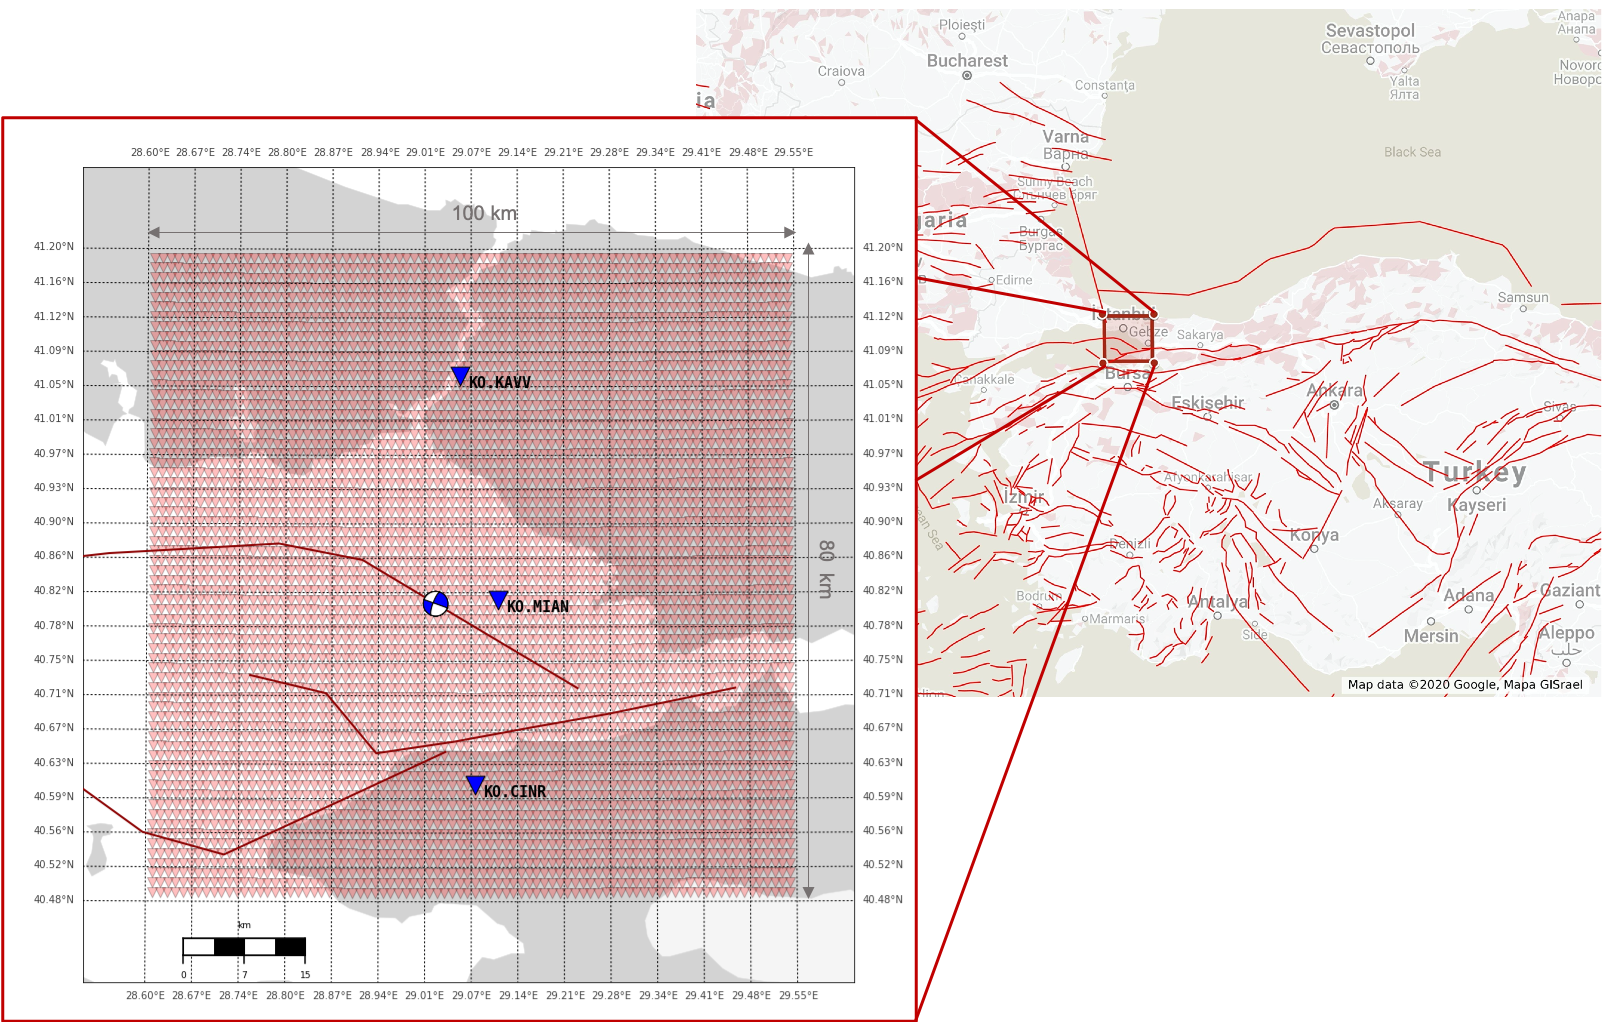
\includegraphics[width=.75\linewidth]{images_methods/Overviewfig_istanbul_domain.png}
    \caption{Overview map of the Istanbul domain. A grid of 5544 receivers is placed over Istanbul and part of the Marmara sea. The initial source is located at the middle of the Princess Island Segment. Crustal fault coordinates from SHARE database \cite{basilic2013european}. Three receivers are selected in the grid, which are closest to real strong motion stations.}
    \label{fig:overviewfig_grid_istanbul}
\end{figure}


\subsection{Short overview workflow}

First a reference configuration and simulation setup is created. We place a grid of receivers of 100 km by 80 km covering the segment of the NAFZ just south of Istanbul, see Figure \ref{fig:overviewfig_grid_istanbul}. Three real stations were selected in this domain, and the closest receiver in the grid is used to simulate the response of these stations for various analyses. The over-all reference set-up is the flat domain, with a 3D volume model. The influence of a domain with a 1D model, with topography and with ocean can then be assessed. Furthermore, individual reference set-ups are created for the 3D, 1D, 3D+topo and 3D+topo+ocean simulations. The variation of source parameters can then be referenced to these four set-ups. 

\subsection{Source parameter variation}

% Please add the following required packages to your document preamble:
% \usepackage{booktabs}
\begin{table}[]
\caption{Initial strike dip and rake of four test CMT configurations and the range over which they are varies.}
\begin{tabular}{@{}l|llll@{}}
\toprule
 & \textbf{Strike{[\degree]}} & \textbf{Dip [$\degree$]} & \textbf{Rake [$\degree$]} & \textbf{Regime} \\ \midrule
\textbf{CMT1} & 90  +/- 45 & 90 -45 & 180 +/- 90 & Dextral strike-slip \\
\textbf{CMT2} & 100 +/- 45 & 75 -45 & 160 +/- 90 & Dextral strike-slip \\
\textbf{CMT3} & 10 +/- 45  & 30 +45 & 90 +/- 90  & Thrust              \\
\textbf{CMT4} & -10 +/- 45 & 60 -45 & -90 +/- 90 & Normal              \\ \bottomrule
\label{tab:CMTstarts}
\end{tabular}
\end{table}


Once the reference set-ups are defined, we generate reference events. This is done via six simulations of unit moment magnitude ($M_0 = 1$ ) for each component, and the other components are set to zero. For moment tensor variations, four CMT solutions were created as a starting point. See Table \ref{tab:CMTstarts} for the initial strike, dip and rake of these solutions. We first start with a simple case: a perfect dextral strike-slip with the fault plane perpendicular to the north. From here we vary up to 50\% of the initial value. This corresponds to 45$\degree$ in the strike, both ways, the dip can only range between 0-90$\degree$, so this is varied only one way. The rake is varied both ways in 90$\degree$. To keep consistent, these values are used for the other CMT starting configurations as well. Subsequently, CMT2 is used as the configuration for a variation in position and depth. As ChEESE works with strike, dip and rake as description of the seismic point source, these are defined for our starting points, and then converted to values for the six individual moment tensor components. After the simulation, the outputs of the six individual simulations are multiplied with their respective values and recombined into the full solution at each receiver in the grid. Separate simulation and re-combination was discussed in  \ref{sec:CMTexplanation}. 

After a full reference solution is computed for each gridpoint for all CMT compositions, the strike, dip and rake are varied and compared to the respective reference set-ups. 
%Figures \hl{ref to figures with strike dip rake variation from each m.t. component to a total solution} show already what happens to the total moment magnitude when these three parameters are varied. 

In the results, the \textit{coefficient of variation} $Cv$ of a proxy is calculated for each gridpoint $i$ and each variation $j$ of strike, dip and rake parameters $p$:

\begin{equation}
Cv_{p, i} = \frac{\sigma_{p, i, j}}{\mu_{i}},
\end{equation}

with $\sigma_{p,i}$ the standard deviation of a parameter $p$ at the grid point $i$ for each variation $j$. This coefficient thus gives a normalised standard deviation over all variations in strike, dip and rake. The relative difference of 15$\degree$ and 22.5$degree$ with respect to the initial CMT is calculated as:

\begin{equation}
    diff_{p,i} = \frac{P_{var} - P_{ref}}{P_{ref}},
\end{equation}

with $P$ the ground motion proxy. This measure gives the factor with which the varied scenario is amplified or de-amplified with respect to the reference CMT.

\subsubsection{Depth and positional variation}

In addition to varying the angle of the strike, dip and rake of the source, depth and position are also shortly evaluated. Position was varied 10km along the strike of the (??) segment of the NABF, towards both sides of the initial location. The depth, as discussed earlier, is one of the least well-constrained parameters in source inversion and characterization. Therefore, a short study on the influence of source depth on the distribution of ground motion is conducted. we vary the source between a depth of 15 km and 5 km, in increments of 2.5 km. 

\subsection{Processing}

The Obspy python package was used for the majority of processing. Comparison between observed and simulated seismograms for model validation can be done when the two signals are adequately processed. In order to compare simulated waveforms to data, the data and simulations must be in the same units and frequency range. Ground motion at strong motion stations is recorded in Counts. Response removal converts Counts to a velocity, acceleration or displacement time-series. This conversion is dependent on the seismometer in question and requires a gain factor, conversion factor and sensitivity. Only complete records with a response file can be converted to a ground motion series. In the case of Turkey numerous stations fail to deliver a response file, rendering a large part of the recorded data unworkable. After response removal the two signals should be filtered to the same frequency bandwidth. We apply a butterworth bandpass filter of $0.01 Hz - f^{max}$ to the simulation and recorded data. Finally, care should be taken when comparing simulations at different frequencies with each other, or with recorded data. The start-time of the signal varies due to the definition of the source-time function (See eq. \ref{eq:Gaussianrate} and \ref{eq:custom}). 

\section{Validation of Model}

To validate that the \textit{csem\_eastmed} model performs well for our purpose, results of simulation of a historic event, using this model, has to be compared with the measured data at the seismometer station locations. Required for this is an event that has a CMT solution published by the GCMT catalogue, is covered by various stations within the range of 200 km, for a reasonable model domain size. The magnitude should be light ($M_w 4.0-4.9$) to moderate ($M_w 5.0-5.9$), to remain within the range of magnitudes that a CMT solution can reasonably describe. 

\begin{figure}
    \centering
    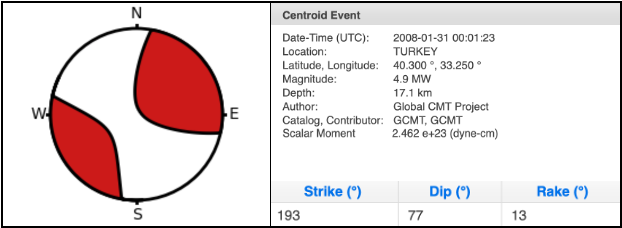
\includegraphics[width=0.4\textwidth]{images_methods/infocubuk.png}
    \caption{Information distributed by the GCMT about the 2008-01-31 00:01:22 UTC Çubuk event.}
    \label{fig:cubukeventinfo}
\end{figure}

The only event in Western Turkey that fulfils these conditions was the 2008-01-31 00:01:22 UTC $Mw 4.9$ event near Çubuk, north-east of Ankara (see Figures \ref{fig:cubuk_domain} and \ref{fig:cubukeventinfo}). From here on, we will name this the $M_w 5.0$ Cubuk event. This earthquake was recorded by the temporary YL array from 2005 - 2008, maintainded by the University of Arizona, and the permanent KOERI array that is mainained by the Bogazici University Kandilli Observatory And Earthquake Research Institute, \cite{https://doi.org/10.7914/sn/ko}. The YL array was set up in the context of the project \textit{Continental lithospheric deformation along a major strike-slip fault zone: the central North Anatolian Fault Zone, Turkey}, \cite{https://doi.org/10.7914/sn/yl_2005}. The stations are broadband (10-80 Hz sampling frequency) high-gain seismometers in E, N and Z orientation: BHE, BHN, BHZ.

Table \ref{Domain parameters of the simulations in Istanbul and Çubuk} shows the parameters for the two domains that were considered for the validation. A large domain containing 37 YL stations, and a smaller sub-domain containing only 7 receivers.  We first selected a large domain of 300 by 120 km containing 37 stations, and simulate the event at periods of 20s, 15s, and 10s. A waveform comparison and goodness-of-fit (GoF) analysis, explained further in the next paragraph, is done for the simulated and real data recorded at the 37 receivers in the domain. 

To mitigate high computational costs, a smaller domain is selected to run the event for periods of 20s, 15s, 10s, 8s, 6s, 4s, 2s, 1s. The waveform data at the receiver locations is then compared to the station data to assess performance for the increasing frequencies. The small domain spans 100 by 80 km and contains seven receivers. 


\begin{figure}
    \centering
    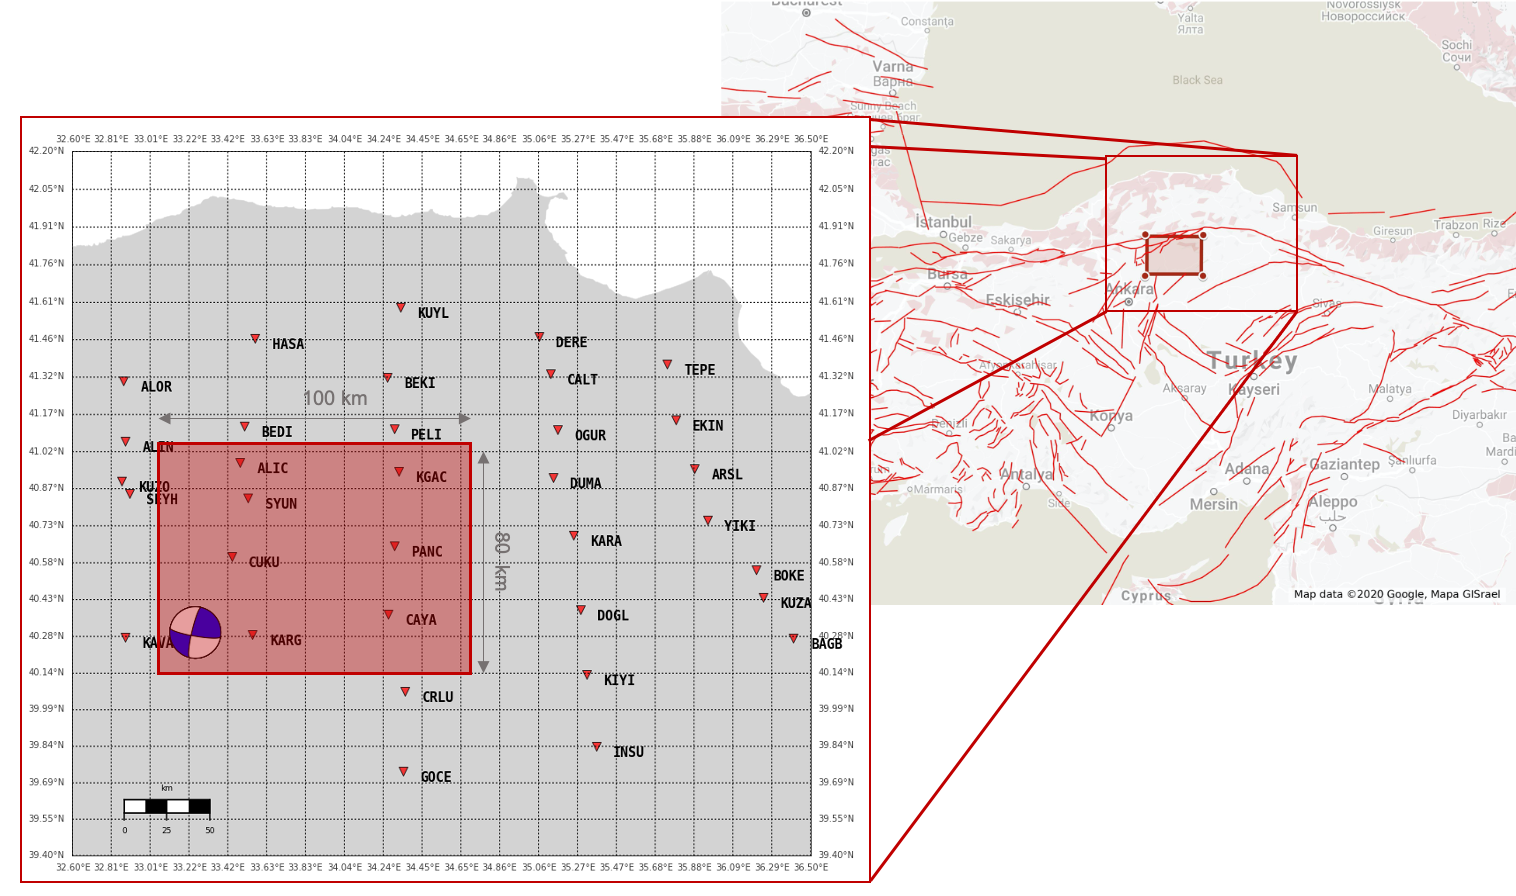
\includegraphics[width=0.75\textwidth]{images_methods/Overviewfig_cubuk_domain.png}
    \caption{Caption}
    \label{fig:cubuk_domain}
\end{figure}



\subsection{Goodness of Fit (GoF)}

Quantifying the amount of agreement between observed and synthetic data can be done with a goodness-of-fit (GoF) analysis. A comparison of 10 criteria was proposed by \cite{anderson_quantitative_nodate}. This GoF analysis rates the performance of the parameter by scoring the fit 1 to 10, with categories poor (0-4), fair (4-6) , good(6-8), excellent (8-10) fit. This is done by comparing between the outcome of one parameter $p_1$ to the outcome of the other parameter $p_2$, in this case data and synthetics:

\begin{equation}
S\left(p_{1}, p_{2}\right)=10 \exp \left\{-\left[\frac{\left(p_{1}-p_{2}\right)}{\min \left(p_{1}, p_{2}\right)}\right]^{2}\right\}.
\end{equation}

The criteria that were used for the validation in the large domain were PGA, PGV, PGD, Arias Intensity, Energy integral. For the smaller domain, the cross-correlation, response spectra and Fourier spectra were also evaluated per frequency. 

\end{document}